\documentclass{article}

\usepackage{amsmath}
\usepackage{graphicx}

\def\I{\overline{I}}
\def\d{\mathrm{d}}
\def\real{\mathrm{Re}}
\def\imag{\mathrm{Im}}

\title{A Brief Derivation for Spatial DFT Extraction from Langmuir Probe Currents}
\author{Christopher R. Martin\\Associate Professor of Mechanical Engineering\\Penn State Altoona}
\date{\today}

\begin{document}

\maketitle

\section{Derivation}

The probe wire has radius, $R$, and rotates about a center on the $x$-axis a distance, $d$, from the origin.  At each sample, the probe will have an angle, $\theta$, will enter the domain at radius, $R_0$, and terminates at a radius, $R_1$.  The current measured by the probe, $I$, is an integral of the current per unit wire length, $\I(r)$,
\begin{align}
I = \int_{R_0}^{R_1} \I(r) \d r.
\end{align}
These dimensions are shown in Figure \ref{fig:coords}.  When the tip of the wire lies inside the domain, $R_1 = R$.

\begin{figure}
\centering
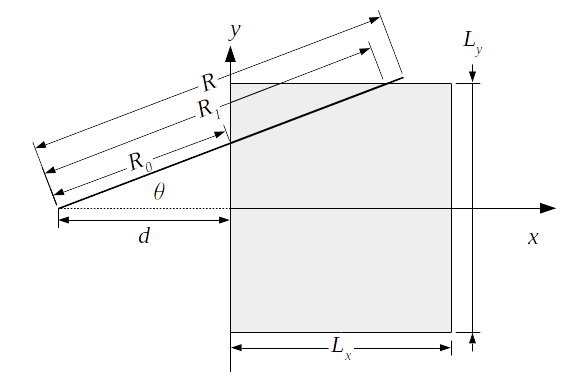
\includegraphics[width=.9\linewidth]{figures/coords}
\caption{Dimensions and coordinate system for the domain}\label{fig:coords}
\end{figure}

In the previous work, $\I$, was calculated as a grid of discrete nodes, and its values along the probe length.  This approach is flexible and intuitive, but inverting this integral for an arbitrary wire location requires a relatively expensive interpolation through each grid square the wire occupies.  

In the present work, we adopt a spatial Fourier series, which provides a far more numerically elegant formulation.

\subsection{Fourier series}

The Fourier series for $\I$ is constructed in $x,y$ coordinates
\begin{align}
\I(x,y) &= \real \sum_{m=0}^{N_x} \sum_{n=0}^{N_y} c_{m,n} \exp\left(2\pi j \left(\frac{mx}{L_x} + \frac{ny}{L_y}\right)\right).
\end{align}
Because $c_{m,n}$ is complex (except for $c_{0,0}$), this formulation has $2(N_x+1)(N_y+1)-1$ independent coefficients, and represents a function with periodicity $L_x$ on $x$ and $L_y$ on $y$.  It is continuous, but can only resolve features on the scale $L_x / N_x$ and $L_y / N_y$.  In this way, it has an effective resolution determined by the $N$ values, not entirely unlike a grid resolution.

\subsection{Evaluating the integral}

The integral of $\I$ requires an $x,y$ parametric formulation of the wire's path.  In this derivation, a number of trigonometric functions will be required, so for compactness of notation, 
\begin{align}
s_\theta &\equiv \sin(\theta)\\
c_\theta &\equiv \cos(\theta)
\end{align}

If $r$ is the distance along the wire from the disc center, the corresponding location in $(x,y)$ is
\begin{align}
x &= r c_\theta - d\\
y &= r s_\theta.
\end{align}
The radius at which the wire crosses into the domain, $R_0$, the radius at which the wire either terminates or leaves the domain, $R_1$, and the wire length in the domain, $\Delta R$, are
\begin{align}
R_0 &= \frac{d}{c_\theta}\\
R_1 &= \min\left(\ R,\ \frac{d + L_x}{c_\theta},\ \left|\frac{L_y}{2s_\theta}\right|\ \right)\\
\Delta R &= R_1 - R_0.
\end{align}
The integral is a sum of surface currents along the wire's length at moment in time, so the disc position parameters, $d$ and $\theta$, are constant.  For compactness of notation, it will become convenient to express the trigonometric functions on $\theta$ as constants, $c_\theta$ and $s_\theta$.

A single term of the Fourier series appears
\begin{align*}
&c_{m,n} \exp\left(2\pi j \left( \frac{m(r c_\theta - d)}{L_x} + \frac{n r s_\theta}{L_y} \right)\right)\\
&= c_{m,n} \exp\left(-2\pi j \frac{md}{L_x} \right) \exp\left(2\pi j \left( \frac{m c_\theta}{L_x} + \frac{n s_\theta}{L_y} \right) r\right)\\
&= c_{m,n} \exp\left(-2\pi j \frac{md}{L_x} \right) \exp\left(2\pi j k r \right)
\end{align*}
The \emph{wavenumber}, $k$, is the frequency (in units 1/length) along the wire's path.  It's definition is
\begin{align}
k = \frac{m c_\theta}{L_x} + \frac{n s_\theta}{L_y}.
\end{align}

For an integral over $r$, all but the last portion of the term above is constant, so it is convenient to define a new parameter, $\gamma$, which represents the value of this term integrated over $r$:
\begin{align}
\gamma_{m,n}(d,\theta) &= \int_{R_0}^{R_1} \exp\left(2\pi j k r \right) \d r \nonumber\\
 &= \left\{\begin{array}{c|l}
 \Delta R & m = n = 0\\
 \frac{1}{2\pi j k}\left[\exp\left(2\pi j k r \right)\right]^{R_1}_{R_0} & \mathrm{otherwise}
\end{array}
\right. .
\end{align}

When we express the complex coefficient, $c_{m,n}$ in its real and imaginary parts,
\begin{align}
c_{m,n} = a_{m,n} + j b_{m,n},
\end{align}
this yields an expression for the total wire current
\begin{align}
I(d,\theta) &= \real \sum_{m=0}^{N_x} \exp\left(-2\pi j \frac{md}{L_x} \right) \sum_{n=0}^{N_y} c_{m,n} \gamma_{m,n} 
\end{align}

The wavenumber, $k$, is repeated here for convenience.  Of course, $\gamma$ could be expressed in terms of sines and cosines, but that is neither cleaner notation, nor more numerically convenient, so we elect to leave the formulation in complex components.

\subsection{Offset current}

Every experiment begins by zeroing the current signal to the nearest practical precision, but no real signal will ever be perfectly zero to numerical precision.  In most applications, this is not especially problematic, but the derivation above makes no allowance for any component of current signal that appears on portions of the wire where $x$ is negative.  For this reason, it is prudent to add a global offset parameter, which is intended to be a small current that is present everywhere.  

\begin{align}
I(d,\theta) &= I_0 + \real \sum_{m=0}^{N_x} \exp\left(-2\pi j \frac{md}{L_x} \right) \sum_{n=0}^{N_y} c_{m,n}\gamma_{m,n}\label{eqn:I}
\end{align}

\section{Inversion}

Fourier transforms classically take advantage of the orthogonality of the sinusoidal basis functions, so the original signal only needs to be integrated against each basis function over the entire domain to calculate the magnitude and phase of that component.  Because no single wire position spans the entire domain, this approach is not tenable.

Instead, we benefit from the fact that the unknown parameters are linear coefficients.  If they were to be serialized in a vector, $\vec{x}$, the problem lends itself to a simple least-squared approach.  Because they are complex each instance of $c_{m,n}$ actually represents two unknown coefficients,
\begin{align}
c_{m,n} = a_{m,n} + j b_{m,n}.
\end{align}
The scheme used to organize the coefficients in $\vec{x}$ is not especially important, but it might be something along the lines of 
\begin{align}
\vec{x} = \{a_{0,0},\ I_0,\ a_{1,0},\ b_{1,0},\ a_{2,0},\ b_{2,0},\ \ldots \}^T.
\end{align}
Note that $b_{0,0}$ has been replaced by the offset current, $I_0$.  When $m=n=0$, the expression is purely real, so $b_{0,0}$ is ignored by this formulation - the solution is independent of its selection.  So, with the addition of $I_0$, there are $2(N_x+1)(N_y+1)$ coefficients to be calculated.

When the terms of (\ref{eqn:I}) are embedded into a second vector, $\vec{\Lambda}$, the equation may be rewritten
\begin{align}
I(d,\theta) = \vec{\Lambda}(d,\theta) \cdot \vec{x}.
\end{align}
Here, $\vec{\Lambda}$, is a vector that models the contribution of each coefficient to the current of a wire in location $(d,\theta)$.

For a given wire position, $(d_i, \theta_i)$, there will be a measured current, $I_i$.  For a given coefficient set, there will be an error,
\begin{align}
e_i = I_i - \vec{\Lambda}(d_i, \theta_i) \cdot \vec{x}.
\end{align}
In a least squares approach, we differentiate the sum of the squares of errors for each of the data points.  For compactness of notation, it will be convenient to abbreviate $\vec{\Lambda}_i = \vec{\Lambda}(d_i, \theta_i)$ moving forward.

\begin{align}
\vec{0} = \nabla \sum e_i {^2} = \sum 2(I_i - \vec{\Lambda}_i \cdot \vec{x})(- \vec{\Lambda}_i)
\end{align}
Solving for $\vec{x}$,
\begin{align}
\vec{x} = \left(\sum \vec{\Lambda}_i \vec{\Lambda}_i{^T}\right)^{-1} \sum I_i \vec{\Lambda}_i
\end{align}

The multiplication of $\Lambda$ with its transpose forms a symmetrical matrix.  The summation accumulate over the body of data collected to form a matrix that must be inverted.

\end{document}
